%% possible_limitations.tex
%% Exploration of potential Phlex limitations and mitigations.
%% Compile with: pdflatex possible_limitations.tex

\documentclass[aspectratio=169,10pt]{beamer}

\usetheme{Boadilla}
\usecolortheme{seahorse}
\setbeamertemplate{navigation symbols}{}
\setbeamerfont{frametitle}{size=\normalsize,series=\bfseries}
\setbeamerfont{framesubtitle}{size=\small}

\usepackage{listings}
\usepackage{xcolor}
\usepackage{booktabs}
\usepackage{array}
\usepackage{microtype}
\usepackage{tikz}
\usetikzlibrary{shapes.geometric,arrows.meta,positioning,fit,backgrounds}

%% ---- code listing style -----------------------------------------------
\lstdefinestyle{cppstyle}{
  language=C++,
  basicstyle=\ttfamily\tiny,
  keywordstyle=\color{blue!70!black}\bfseries,
  commentstyle=\color{gray!70},
  stringstyle=\color{green!50!black},
  numbers=none,
  breaklines=true,
  showstringspaces=false,
  frame=single,
  frameround=tttt,
  backgroundcolor=\color{gray!8},
  xleftmargin=4pt, xrightmargin=4pt,
  aboveskip=4pt, belowskip=2pt,
}
\lstset{style=cppstyle}

%% ---- colour helpers ----------------------------------------------------
\newcommand{\good}[1]{\textcolor{green!50!black}{\textbf{#1}}}
\newcommand{\bad}[1]{\textcolor{red!70!black}{\textbf{#1}}}
\newcommand{\warn}[1]{\textcolor{orange!80!black}{\textbf{#1}}}
\newcommand{\corr}[1]{\colorbox{yellow!30}{\textbf{#1}}}
\newcommand{\code}[1]{\texttt{\small #1}}

%% -----------------------------------------------------------------------
\title{Possible Phlex Limitations}
\subtitle{Exploration, Refutations, and Mitigations}
\author{Brett Viren}
\date{2026}

%% =======================================================================
\begin{document}

\begin{frame}
  \titlepage
  \begin{block}{Purpose}
    Each possible limitation is examined against the actual source code.
    Misunderstandings are refuted before mitigations are discussed.
  \end{block}
\end{frame}

%% -----------------------------------------------------------------------
%% LIMITATION 1
%% -----------------------------------------------------------------------

\begin{frame}{Limitation~1 --- The Chunked Stream Problem (Overview)}
  \framesubtitle{Also known as overlap-add / overlap-save convolution}

  \textbf{Setting:} An ``event'' data cell holds a long time-series waveform.
  The waveform is too large to fit in RAM as a single product, so it is split
  into overlapping \emph{fragments} (chunks) in a child layer.

  \medskip
  \begin{columns}[T]
    \begin{column}{0.48\textwidth}
      \textbf{Required computation} \\[2pt]
      \begin{itemize}\small
        \item FFT-based convolution (or deconvolution) whose kernel is
              shorter than the fragment but whose impulse response extends
              across fragment boundaries.
        \item Each algorithm invocation must see fragment $N$ \emph{and} the
              saved ``tail'' from fragment $N{-}1$ (overlap-add) or a
              ``lookahead'' from fragment $N{+}1$ (overlap-save).
        \item The partial result of fragment $N$ must be stored and applied
              when processing fragment $N{+}1$.
      \end{itemize}
    \end{column}
    \begin{column}{0.48\textwidth}
      \textbf{What the data-layer model guarantees} \\[2pt]
      \begin{itemize}\small
        \item Each algorithm invocation receives the product stores of
              \emph{exactly the cells it was wired to receive}
              (one cell per transform invocation; many cells only via fold).
        \item No sliding-window primitive exists.
        \item No guaranteed delivery order of fragments from the
              \code{index\_router} $\to$ provider $\to$ transform chain.
        \item Fold accumulates all fragments before emitting --- requires
              all fragments to fit in RAM simultaneously.
      \end{itemize}
    \end{column}
  \end{columns}

  \medskip
  \begin{alertblock}{Verdict}
    This is a \bad{real gap}.  The Phlex data model is designed for
    cell-independent algorithms.  Temporal dependency between sibling cells
    requires explicit work-arounds at the algorithm or framework level.
  \end{alertblock}
\end{frame}

%% -----------------------------------------------------------------------

\begin{frame}[fragile]{Limitation~1 --- Available Mechanisms Today}
  \framesubtitle{Three patterns that can express overlap-add in Phlex}

  \begin{columns}[T]
    \begin{column}{0.48\textwidth}
      \textbf{Pattern A: Stateful algorithm object} \\[2pt]
      \small
      Register a stateful class whose member function is called once per
      fragment.  The object holds the tail buffer across calls.
      \begin{lstlisting}
auto obj = g.make<OvlapAdd>(kernel);
obj.transform("conv_step",
  &OvlapAdd::process,
  concurrency::serial);   // REQUIRED
      \end{lstlisting}
      \begin{itemize}\tiny
        \item \good{Works} if fragments arrive in index order.
        \item \warn{Requires} \code{concurrency::serial} to prevent
              simultaneous invocations (mutual exclusion, not ordering).
        \item \bad{No ordering guarantee} --- see next slide.
      \end{itemize}
    \end{column}
    \begin{column}{0.48\textwidth}
      \textbf{Pattern B: Fold with in-memory accumulation} \\[2pt]
      \small
      Fold accumulates all fragments at the event level, then emits one
      result.
      \begin{itemize}\tiny
        \item \good{Ordering handled} by the fold's flush mechanism.
        \item \bad{All fragments must fit in RAM simultaneously} ---
              defeats the purpose of chunking for large events.
      \end{itemize}

      \medskip
      \textbf{Pattern C: Layered unfold + fold pipeline} \\[2pt]
      \small
      Unfold creates \code{fft\_block} grandchildren; transform per
      block; fold assembles blocks back to fragment result.
      \begin{itemize}\tiny
        \item \good{Decomposes} the computation into fine-grained cells.
        \item \warn{Overlap tail} still requires state across sequential
              fragment invocations --- reduces to Pattern A for the
              inter-fragment step.
        \item \bad{Same ordering problem} applies at the fragment level.
      \end{itemize}
    \end{column}
  \end{columns}
\end{frame}

%% -----------------------------------------------------------------------

\begin{frame}{Limitation~1 --- The Index-Ordering Problem}
  \framesubtitle{Why \texttt{concurrency::serial} is necessary but not sufficient}

  \begin{alertblock}{Key finding (from \texttt{index\_router} and TBB)}
    The \code{index\_router} delivers indices via TBB's
    \code{flow::graph}, which makes \bad{no ordering guarantees}.
    \code{concurrency::serial} ensures \emph{mutual exclusion}
    (at most one invocation at a time) but \emph{not execution order}.
    Fragments may arrive at the algorithm object in any sequence.
  \end{alertblock}

  \medskip
  \begin{columns}[T]
    \begin{column}{0.38\textwidth}
      \textbf{Severity} \\[4pt]
      \small
      For overlap-add to be mathematically correct, fragment $N$ must be
      processed \emph{before} fragment $N{+}1$.  Out-of-order processing
      produces wrong results silently --- no error is raised.
    \end{column}
    \begin{column}{0.58\textwidth}
      \textbf{Mitigation at the algorithm level} \\[4pt]
      \small
      \begin{enumerate}
        \item \textbf{Sequence-number buffer}: the algorithm object maps
              fragment number $\to$ fragment data.  It processes
              fragments in ascending order once the expected fragment
              arrives, queuing out-of-order ones.
        \item \textbf{Lazy emission}: the algorithm defers output until
              it has confirmed no gap precedes the current fragment.
        \item \textbf{Driver ordering contract}: the driver emits
              fragment indices in ascending order \emph{and} the TBB
              graph happens to deliver them in FIFO order for a serial
              chain.  \warn{Fragile:} depends on undocumented TBB
              scheduler behaviour.
      \end{enumerate}
    \end{column}
  \end{columns}

  \medskip
  \begin{exampleblock}{Mitigation at the framework level (proposed)}
    A \textbf{sequencing node} primitive --- a TBB buffer that re-orders
    incoming messages by \code{data\_cell\_index::number()} before
    forwarding them --- would make Pattern~A safe without requiring
    algorithm-level buffering.
  \end{exampleblock}
\end{frame}

%% -----------------------------------------------------------------------

\begin{frame}{Limitation~1 --- Proposed Framework Enhancements}
  \framesubtitle{What Phlex could add to support chunked stream algorithms natively}

  \begin{columns}[T]
    \begin{column}{0.48\textwidth}
      \textbf{Enhancement 1: Sequencing node} \\[2pt]
      \small
      A new node type \code{sequenced\_transform} that buffers messages
      from a child layer and delivers them in ascending
      \code{data\_cell\_index::number()} order before invoking the
      algorithm.  Minimal API change; wraps TBB
      \code{sequencer\_node}.
      \begin{itemize}\tiny
        \item Eliminates algorithm-level sorting.
        \item Requires a ``successor number'' state per parent cell ---
              flushed when a flush message arrives.
      \end{itemize}
    \end{column}
    \begin{column}{0.48\textwidth}
      \textbf{Enhancement 2: Sliding-window fold} \\[2pt]
      \small
      A new fold variant that holds a window of $W$ consecutive cells
      and invokes the algorithm once per window position, advancing by
      $S$ cells (stride).  Emits results at the child layer (same layer
      as inputs).
      \begin{itemize}\tiny
        \item Naturally expresses overlap-add: $W=2$ fragments,
              $S=1$ fragment.
        \item Requires ordering guarantee (Enhancement~1 first).
        \item Output layer and input layer are the same --- currently
              unsupported fanout pattern (see Limitation~1 Slide~Q7).
      \end{itemize}
    \end{column}
  \end{columns}

  \bigskip
  \begin{block}{Summary for Limitation~1}
    \small
    \begin{tabular}{@{}lll@{}}
      \toprule
      Approach & Works today? & Caveats \\
      \midrule
      Stateful object + serial concurrency & \warn{With care} & No order guarantee \\
      Stateful object + index-sorted buffer & \good{Yes} & Algorithm complexity \\
      Fold (all fragments in RAM) & \bad{Too large} & Defeats chunking purpose \\
      Sequencing node (proposed) & Future & Framework change needed \\
      Sliding-window fold (proposed) & Future & Framework change needed \\
      \bottomrule
    \end{tabular}
  \end{block}
\end{frame}

%% -----------------------------------------------------------------------
%% LIMITATION 2
%% -----------------------------------------------------------------------

\begin{frame}{Limitation~2 --- Hierarchy-Algorithm Collusion (Stated Concern)}
  \framesubtitle{Must unfold child layers be pre-declared in \texttt{fixed\_hierarchy}?}

  \textbf{The concern:}  When an algorithm uses \code{unfold} to create
  child data cells in a new layer (e.g.\ \code{"fragment"}), every other
  part of the system that defines or validates the hierarchy must also
  mention \code{"fragment"}.  If true, this would require a tight collusion
  between:

  \begin{itemize}
    \item The driver plugin (which provides \code{fixed\_hierarchy}).
    \item Every algorithm plugin that unfolds into or consumes from that layer.
    \item Any configuration layer that assembles the workflow.
  \end{itemize}

  \medskip
  \textbf{Example scenario:}

  \begin{columns}[T]
    \begin{column}{0.48\textwidth}
      \small
      Driver declares:
      \begin{itemize}\small
        \item \code{fixed\_hierarchy\{\{"\!run"\}, \{"\!run", "\!event"\}\}}
      \end{itemize}
      Algorithm ``splitter'' unfolds \code{"event"} $\to$
      \code{"my-special-layer-of-parts"}.

      \medskip
      \textbf{Question:} must \code{"my-special-layer-of-parts"} appear in
      the driver's \code{fixed\_hierarchy}?
    \end{column}
    \begin{column}{0.48\textwidth}
      \small
      Downstream algorithm ``process-part'' queries:
      \begin{lstlisting}
product_query{.creator = "splitter",
              .layer   = "my-special-layer-of-parts"}
      \end{lstlisting}
      \textbf{Question:} does \code{edge\_maker} need the layer in
      \code{fixed\_hierarchy} to wire this edge?
    \end{column}
  \end{columns}
\end{frame}

%% -----------------------------------------------------------------------

\begin{frame}[fragile]{Limitation~2 --- \corr{Refutation}: Unfold Bypasses \texttt{fixed\_hierarchy}}
  \framesubtitle{The unfold calls \texttt{make\_child()} directly, not through the validated cursor}

  \begin{alertblock}{\corr{Key finding} --- this concern is largely a non-issue}
    An \code{unfold} creates child indices by calling
    \code{data\_cell\_index::make\_child()} directly
    (\texttt{declared\_unfold.hpp:170}).
    This \bad{bypasses} \code{data\_cell\_cursor::yield\_child()}, which is
    the only path that calls \code{fixed\_hierarchy::validate()}.
    No validation error is raised for layers not in \code{fixed\_hierarchy}.
  \end{alertblock}

  \begin{columns}[T]
    \begin{column}{0.50\textwidth}
      \textbf{Two distinct hierarchy objects} in \code{framework\_graph}:
      \begin{lstlisting}
// framework_graph.hpp:157-158
fixed_hierarchy  fixed_hierarchy_; // validates driver yields only
data_layer_hierarchy hierarchy_{};  // observes ALL layers (no validation)
      \end{lstlisting}
      \begin{itemize}\small
        \item \code{fixed\_hierarchy\_} is only enforced via
              \code{data\_cell\_cursor::yield\_child()} in the driver.
        \item \code{data\_layer\_hierarchy} (the observer) receives indices
              from both the driver source AND unfold output via
              \code{hierarchy\_node\_} --- no validation performed
              (\texttt{framework\_graph.cpp:41--46}).
      \end{itemize}
    \end{column}
    \begin{column}{0.46\textwidth}
      \textbf{Unfold index emission path} (bypasses validation):
      \begin{lstlisting}
// declared_unfold.hpp:170,182-185
auto new_id = unfolded_id->make_child(
    child_layer(), counter);  // no validate()

auto child = g.make_child_for(
    counter++, std::move(new_products));
// port 1: raw index to hierarchy_node
tbb::flow::output_port<1>(unfold_).try_put(
    child->index());
      \end{lstlisting}
      \begin{itemize}\small
        \item \code{index\_router} has no reference to
              \code{fixed\_hierarchy} --- it routes by layer hash
              regardless of whether the layer was pre-declared.
      \end{itemize}
    \end{column}
  \end{columns}
\end{frame}

%% -----------------------------------------------------------------------

\begin{frame}[fragile]{Limitation~2 --- What Collusion IS Real}
  \framesubtitle{An implicit string-naming contract between plugins}

  Although \code{fixed\_hierarchy} does not constrain unfold child layers,
  a different and \warn{real} form of collusion exists:

  \begin{columns}[T]
    \begin{column}{0.48\textwidth}
      \textbf{String-name contract} \\[2pt]
      \small
      The unfold plugin names the child layer at registration time:
      \begin{lstlisting}
g.unfold<Splitter>("splitter", pred, unf,
    "my-special-layer-of-parts");
      \end{lstlisting}
      Any downstream algorithm that consumes from this layer must use
      the identical string in its \code{product\_query}:
      \begin{lstlisting}
product_query{.creator = "splitter",
  .layer = "my-special-layer-of-parts"}
      \end{lstlisting}
      \begin{itemize}\tiny
        \item If the strings differ, \code{edge\_maker} reports a
              configuration error at \code{finalize()} time --- not at
              runtime.
        \item \good{Caught at startup}: any mismatch is a hard error
              before the first data cell is emitted.
      \end{itemize}
    \end{column}
    \begin{column}{0.48\textwidth}
      \textbf{Fold flush-source collusion} \\[2pt]
      \small
      A fold that consumes from an unfold's child layer must receive
      flush messages from the \emph{unfold's flusher}, not the
      graph-wide flusher.  Phlex wires this automatically
      (\texttt{framework\_graph.cpp:150--172}):
      \begin{lstlisting}
// automatically connects unfold flusher
// to any fold consuming its child layer
if (auto it = unfold_flushers.find(pq.layer);
    it != unfold_flushers.end()) {
  flushers.insert(it->second);  // unfold flusher
} else {
  flushers.insert(&index_router_.flusher());
}
      \end{lstlisting}
      \begin{itemize}\tiny
        \item \good{Automatic}: user does not wire this manually.
        \item The layer-name string is the key for this lookup too ---
              same contract as above.
      \end{itemize}
    \end{column}
  \end{columns}

  \medskip
  \begin{exampleblock}{Summary}
    The \code{fixed\_hierarchy} in the driver does NOT need to mention unfold
    child layers.  The only real collusion is a shared layer-name string
    between the unfold plugin and any downstream consumer, caught as a hard
    error at graph finalization.
  \end{exampleblock}
\end{frame}

%% -----------------------------------------------------------------------

\begin{frame}{Limitation~2 --- Framework Support for the Naming Contract}
  \framesubtitle{What Phlex provides and what is left to the configuration layer}

  \begin{columns}[T]
    \begin{column}{0.48\textwidth}
      \textbf{What Phlex enforces automatically} \\[4pt]
      \small
      \begin{itemize}
        \item[\good{$\checkmark$}] Driver-yielded layers validated against
              \code{fixed\_hierarchy} at \code{yield\_child()} time.
        \item[\good{$\checkmark$}] Unfold child-layer name propagated
              to \code{edge\_maker} automatically from the
              \code{destination\_data\_layer} argument.
        \item[\good{$\checkmark$}] Flush source wired automatically:
              folds consuming an unfold child layer get the unfold's
              flusher, not the global one.
        \item[\good{$\checkmark$}] Unresolved \code{product\_query}
              (no producer found) is a hard error at
              \code{finalize()} --- before execution begins.
      \end{itemize}
    \end{column}
    \begin{column}{0.48\textwidth}
      \textbf{What the configuration layer must assure} \\[4pt]
      \small
      \begin{itemize}
        \item[\warn{User}] The layer-name string used in
              \code{unfold()} and in downstream \code{product\_query}
              fields must match.  This is a shared constant --- best
              placed in a header.
        \item[\warn{User}] The driver's \code{fixed\_hierarchy} should
              list only layers the \emph{driver} itself yields.
              Unfold child layers are not the driver's concern.
        \item[\warn{User}] When using \code{layer\_generator} as a
              factory, only the driver's layers need to be registered
              with \code{add\_layer()}.
      \end{itemize}
      \medskip
      \small\textbf{Separate plugin types} enforce separation of concerns:
      \begin{itemize}\small
        \item \code{PHLEX\_REGISTER\_PROVIDERS} ---
              only \code{provide()} accessible.
        \item \code{PHLEX\_REGISTER\_ALGORITHMS} ---
              \code{fold/transform/unfold/observe} accessible;
              \code{provide()} is \emph{not}.
      \end{itemize}
    \end{column}
  \end{columns}
\end{frame}

%% -----------------------------------------------------------------------
%% LIMITATION 3
%% -----------------------------------------------------------------------

\begin{frame}{Limitation~3 --- The Event Stream Pattern (Overview)}
  \framesubtitle{Time-ordered asynchronous streams with variable-interval data units}

  \textbf{Setting:} Multiple independent hardware streams each produce
  time-stamped data \emph{units}.  Each unit spans a time interval
  $[t_{\mathrm{start}}, t_{\mathrm{end}})$.  There are gaps between
  units.  No synchronisation between streams other than a common clock.

  \medskip
  \begin{columns}[T]
    \begin{column}{0.52\textwidth}
      \textbf{Stream structure} \\[4pt]
      \small
      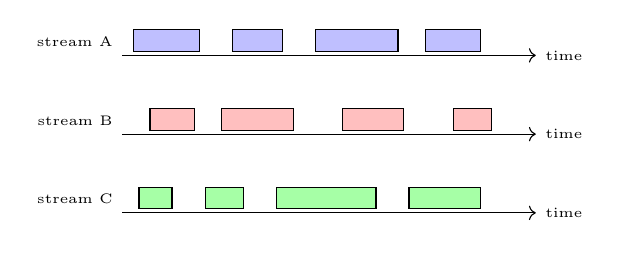
\begin{tikzpicture}[x=0.7cm,y=0.5cm]
        \draw[->] (0,0) -- (7.5,0) node[right]{\tiny time};
        \foreach \x/\w in {0.2/1.2, 2.0/0.9, 3.5/1.5, 5.5/1.0}
          \draw[fill=blue!25] (\x,0.1) rectangle (\x+\w,0.65);
        \node[left] at (0,0.35) {\tiny stream A};
        \begin{scope}[yshift=-1cm]
          \draw[->] (0,0) -- (7.5,0) node[right]{\tiny time};
          \foreach \x/\w in {0.5/0.8, 1.8/1.3, 4.0/1.1, 6.0/0.7}
            \draw[fill=red!25] (\x,0.1) rectangle (\x+\w,0.65);
          \node[left] at (0,0.35) {\tiny stream B};
        \end{scope}
        \begin{scope}[yshift=-2cm]
          \draw[->] (0,0) -- (7.5,0) node[right]{\tiny time};
          \foreach \x/\w in {0.3/0.6, 1.5/0.7, 2.8/1.8, 5.2/1.3}
            \draw[fill=green!35] (\x,0.1) rectangle (\x+\w,0.65);
          \node[left] at (0,0.35) {\tiny stream C};
        \end{scope}
      \end{tikzpicture}
    \end{column}
    \begin{column}{0.44\textwidth}
      \textbf{Three primary operations needed} \\[4pt]
      \small
      \begin{enumerate}
        \item \textbf{Merge streams}: combine $N$ streams into a single
              time-ordered sequence (ordered by unit start time).
        \item \textbf{Merge overlapping units}: when two units from
              different streams (or same stream) overlap in time, combine
              them into one unit.
        \item \textbf{Fragment to fixed blocks}: split each (possibly
              large) unit into fixed-duration sub-units, producing a
              ``chunked stream with gaps'' --- the Limitation~1 pattern.
      \end{enumerate}
    \end{column}
  \end{columns}

  \medskip
  \begin{alertblock}{Fundamental gap}
    Phlex's data model encodes cell identity as a bare \code{size\_t}
    number with no temporal semantics.  There is no timestamp field in
    \code{data\_cell\_index}, \code{product\_store}, or any message type.
    All three operations above require time-based comparison.
  \end{alertblock}
\end{frame}

%% -----------------------------------------------------------------------

\begin{frame}[fragile]{Limitation~3 --- Phlex Assessment per Operation}
  \framesubtitle{Examining each event-stream operation against available primitives}

  \small
  \begin{tabular}{@{}p{0.17\textwidth}p{0.30\textwidth}p{0.46\textwidth}@{}}
    \toprule
    \textbf{Operation} & \textbf{Phlex mechanism} & \textbf{Assessment} \\
    \midrule
    Merge $N$ streams into one time-ordered sequence
    &
    No native merge.  A fold at the parent level can accumulate units
    from all stream data cells.
    &
    \bad{Requires all units in RAM.}
    No streaming merge.
    Time ordering must be implemented by the algorithm (sort by timestamp
    stored in a product).
    The fold's flush fires once --- no incremental output.
    \\[4pt]
    \midrule
    Merge overlapping units
    &
    No native overlap detection.
    Overlap logic must live inside a fold accumulator or a stateful
    transform.
    &
    \bad{No time concept in data model.}
    Must store start/end timestamps as products and implement
    interval-overlap logic in the algorithm.
    All candidates must be present simultaneously.
    \\[4pt]
    \midrule
    Fragment unit to fixed blocks
    &
    \code{unfold}: one unit cell $\to$ many fragment child cells.
    &
    \good{Best fit.}
    The unfold function knows the unit's duration (from a product)
    and emits one child per fixed-size block.
    Produces a chunked stream --- now the Limitation~1 problem.
    \\[4pt]
    \midrule
    Incremental (streaming) processing
    &
    No streaming or lazy-evaluation primitives.
    All products for a cell are in RAM before downstream nodes run.
    &
    \bad{Fundamental mismatch.}
    Event stream processing is inherently incremental; Phlex is
    batch-per-cell.
    \\
    \bottomrule
  \end{tabular}
\end{frame}

%% -----------------------------------------------------------------------

\begin{frame}{Limitation~3 --- Working Approaches Within Current Phlex}
  \framesubtitle{What can be done today, and at what cost}

  \begin{columns}[T]
    \begin{column}{0.48\textwidth}
      \textbf{Approach A: Timestamp-in-product + fold}
      \small
      \begin{enumerate}
        \item Provider reads each stream unit; stores a
              \code{TimeInterval\{t\_start, t\_end\}} product in the
              stream data cell.
        \item A fold at the job level accumulates all stream cells.
              On flush, it: \\
              (a) sorts by \code{t\_start}; \\
              (b) merges overlapping intervals; \\
              (c) emits merged ``event'' cells.
        \item An unfold on each merged event creates fragment cells.
      \end{enumerate}
      \warn{Limitation:} all stream data must fit in RAM.
      Suitable for offline processing of bounded datasets.
    \end{column}
    \begin{column}{0.48\textwidth}
      \textbf{Approach B: Pre-sorted driver}
      \small
      \begin{enumerate}
        \item The driver plugin reads all stream metadata (timestamps),
              performs the merge and overlap-detection offline, and
              then yields pre-assigned ``event'' indices.
        \item Providers receive event indices and serve the relevant
              stream fragments.
      \end{enumerate}
      \warn{Limitation:} requires a two-pass architecture (metadata
      pass then data pass) and couples the driver to all stream sources.
      \good{Advantage:} algorithms stay simple; ordering is guaranteed
      by the driver.
    \end{column}
  \end{columns}

  \medskip
  \begin{exampleblock}{Proposed framework enhancements}
    \small
    \begin{enumerate}
      \item \textbf{Temporal key on data cell}: add an optional
            \code{time\_interval} field to \code{data\_cell\_index} or
            as a mandatory product for stream-layer data cells.
            Phlex could then provide a \code{temporal\_fold} that
            delivers cells in time order and triggers on an overlap
            predicate.
      \item \textbf{Streaming fold / generator}: a new primitive that
            emits results incrementally as new stream data arrive,
            rather than waiting for a global flush.  This would require
            a weaker flush model (``emit when leading edge advances'').
    \end{enumerate}
  \end{exampleblock}
\end{frame}

%% -----------------------------------------------------------------------

\begin{frame}{Limitation~3 --- Summary and Design Tension}
  \framesubtitle{Batch-per-cell vs.\ streaming processing}

  \begin{columns}[T]
    \begin{column}{0.52\textwidth}
      \textbf{Root cause of the limitation} \\[4pt]
      \small
      Phlex's data model is fundamentally \emph{batch-per-cell}: a data
      cell must be fully constituted before downstream algorithms can run.
      Products are immutable once in a store.  This is an excellent fit
      for HEP data where event boundaries are clear and data fits in
      per-event RAM budgets.

      \medskip
      The event stream pattern requires \emph{incremental, time-ordered}
      processing where:
      \begin{itemize}\small
        \item cell boundaries are not known in advance,
        \item ordering by a real-valued timestamp is essential,
        \item partial results must be emitted as new data arrives.
      \end{itemize}
      These properties are in direct tension with the current model.
    \end{column}
    \begin{column}{0.44\textwidth}
      \textbf{Verdict table} \\[4pt]
      \small
      \begin{tabular}{@{}lc@{}}
        \toprule
        Operation & Phlex support \\
        \midrule
        Merge $N$ streams (offline) & \warn{Fold + sort} \\
        Merge $N$ streams (online) & \bad{None} \\
        Overlap detection & \warn{Algorithm only} \\
        Fragment to blocks & \good{Unfold} \\
        Ordered delivery & \bad{None native} \\
        Incremental output & \bad{None} \\
        \bottomrule
      \end{tabular}

      \medskip
      \textbf{Recommendation} \\[4pt]
      \small
      For current Phlex: use Approach~B (pre-sorted driver) for offline
      datasets.  For online streaming use cases, the framework would need
      a temporal-key extension and a streaming fold primitive --- a
      non-trivial but well-defined enhancement.
    \end{column}
  \end{columns}
\end{frame}

%% -----------------------------------------------------------------------
\begin{frame}{Overall Limitation Summary}
  \small
  \begin{tabular}{@{}p{0.20\textwidth}p{0.32\textwidth}p{0.18\textwidth}p{0.20\textwidth}@{}}
    \toprule
    \textbf{Limitation} & \textbf{Root cause} & \textbf{Severity} & \textbf{Best mitigation today} \\
    \midrule
    Chunked stream / overlap-add
    & No sliding-window primitive; no ordering guarantee
    & \warn{Moderate}
    & Stateful object + index-sorted buffer in algorithm \\[4pt]
    Hierarchy-algorithm collusion
    & \corr{Largely a non-issue}: unfold bypasses \code{fixed\_hierarchy}; only string-name contract remains
    & \good{Low}
    & Shared layer-name constant in a header; \code{finalize()} catches mismatches \\[4pt]
    Event stream processing
    & No time concept in data model; batch-per-cell architecture
    & \bad{High} (for streaming use cases)
    & Pre-sorted driver (offline); temporal-key extension (proposed) \\
    \bottomrule
  \end{tabular}

  \bigskip
  \begin{block}{What all three limitations share}
    They each require \emph{ordering} or \emph{comparison} of data cells
    by a key other than the structural \code{(layer, number)} pair.
    A general enhancement would be an \textbf{ordered-delivery guarantee}
    and/or an \textbf{optional cell metadata field} (e.g.\ a real-valued
    timestamp or sort key) that Phlex-native primitives could exploit.
  \end{block}
\end{frame}

\end{document}
